\documentclass{beamer}

% Theme selection
\usetheme{Dresden} % Or any other theme you prefer
\usecolortheme{beaver} % Or any other color theme
\usefonttheme{structuresmallcapsserif}

% Packages
\usepackage[utf8]{inputenc}
\usepackage{amsmath, amssymb}
\usepackage{graphicx}
\usepackage{hyperref}
\usepackage{subcaption}
\usepackage{listings} % For code snippets
\usepackage{ragged2e} % For justified text

% Listing style for code snippets
\lstdefinestyle{mystyle}{
    backgroundcolor=\color{backcolour},
    commentstyle=\color{codegreen},
    keywordstyle=\color{magenta},
    numberstyle=\tiny\color{codegray},
    stringstyle=\color{codepurple},
    basicstyle=\ttfamily\footnotesize,
    breakatwhitespace=false,
    breaklines=true,
    captionpos=b,
    keepspaces=true,
    numbers=left,
    numbersep=5pt,
    showspaces=false,
    showstringspaces=false,
    showtabs=false,
    tabsize=2
}
\lstset{style=mystyle}

% Define colors if not already defined by theme
\definecolor{codegreen}{rgb}{0,0.6,0}
\definecolor{codegray}{rgb}{0.5,0.5,0.5}
\definecolor{codepurple}{rgb}{0.58,0,0.82}
\definecolor{backcolour}{rgb}{0.95,0.95,0.92}

% Title page details
\title{Compressive Sensing with Applications to Near-Field to Far-Field Antenna Pattern Extrapolation}
\author{Jonas Thalmeier}
\institute{EURECOM}
\date{June 20, 2025}

\begin{document}

% Title Slide
\begin{frame}
    \titlepage
\end{frame}

% Table of Contents (Optional, but useful for longer presentations)
\begin{frame}{Outline}
    \tableofcontents
\end{frame}

% Introduction & Project Overview
\section{Introduction}
\begin{frame}{Introduction & Project Overview}
    \begin{itemize}
        \item \textbf{Compressive Sensing (CS):} A signal processing technique for recovering sparse signals from undersampled measurements. 
        \item \textbf{Problem Statement:} Near-field to Far-field Antenna Pattern Extrapolation.
        \item \textbf{Project Goal:} Apply compressive sensing methods to improve antenna measurement techniques through efficient data acquisition and accurate field reconstruction. 
        \item \textbf{Supervisors:} Prof. Dirk Slock, Dr. Zilu Zhao, and Dr. Fangqing Xiao. 
    \end{itemize}
\end{frame}

% Theoretical Foundations
\section{Theoretical Foundations}
\begin{frame}{Sparse Bayesian Learning (SBL)}
    \begin{itemize}
        \item \textbf{Core Idea:} Inducing sparsity in weight vectors through an evidence maximization over a parameterized Gaussian prior. 
        \item \textbf{Observation Model:} $\mathbf{t} = \Phi \mathbf{w} + \boldsymbol{\epsilon}$, where $\boldsymbol{\epsilon} \sim \mathcal{N}(0, \sigma^2 \mathbf{I})$. 
        \item \textbf{Prior:} $p(\mathbf{w} ; \boldsymbol{\gamma}) =\prod\limits^M_{i=1}(2\pi\gamma_i)^{-\frac{1}{2}}\exp (-\frac{w_i^2}{2\gamma_i})$. 
        \item Hyperparameters $\boldsymbol{\gamma}$ inferred via Type-II maximum likelihood. 
    \end{itemize}
\end{frame}

\begin{frame}{EM-Based SBL and its Scalability}
    \begin{itemize}
        \item \textbf{EM Algorithm:} Alternates between E-step (posterior computation) and M-step (hyperparameter update). 
            \begin{itemize}
                \item E-step: $\boldsymbol{\Sigma}_w = \left( \beta \Phi^\top \Phi + \mathrm{diag}(\boldsymbol{\gamma}^{-1}) \right)^{-1}$, $\boldsymbol{\mu}_w = \beta \boldsymbol{\Sigma}_w \Phi^\top \mathbf{t}$. 
                \item M-step: $\gamma_i = \mu_{w,i}^2 + (\Sigma_w)_{ii}$. 
            \end{itemize}
        \item \textbf{Limitation:} High computational cost due to $D \times D$ matrix inversion in each iteration. 
        \item \textbf{Covariance-Free EM (CoFEM):}
            \begin{itemize}
                \item Avoids explicit posterior covariance computation. 
                \item Estimates statistics using linear systems and Rademacher probe vectors. 
            \end{itemize}
    \end{itemize}
\end{frame}

\begin{frame}{Stein's Unbiased Risk Estimate (SURE)}
    \begin{itemize}
        \item \textbf{Stein's Lemma:} Relates expectation of a function of a Gaussian variable to its derivative. 
        \item \textbf{SURE Principle:} Provides an unbiased estimator for the risk ($\mathbb{E}\|\boldsymbol{\mu} - \boldsymbol{\hat{\mu}}\|_2^2$) without knowing the true mean $\boldsymbol{\mu}$. 
        \item \textbf{Application:} Enables hyperparameter optimization by minimizing the SURE. 
            \begin{equation*}
                \hat{\lambda} = \underset{\lambda \in \Lambda}{\arg\min} \left( \|\mathbf{y} - \boldsymbol{\hat{\mu}}_\lambda\|_2^2 + 2\sigma^2 \sum_{i=1}^n \frac{\partial \hat{\mu}_{\lambda,i}}{\partial y_i}(\mathbf{y}) \right) \label{eq:SURE_opt}
            \end{equation*}
    \end{itemize}
\end{frame}

% Algorithm Implementation
\section{Algorithm Implementation}
\begin{frame}{Synthetic Data Generation}
    \begin{itemize}
        \item Generated data using a standard compressive sensing model: $\mathbf{t} = \Phi \mathbf{w} + \mathbf{e}$. 
        \item Components:
            \begin{itemize}
                \item Measurement vector $\mathbf{t} \in \mathbb{R}^N$. 
                \item Sensing matrix $\Phi \in \mathbb{R}^{N \times D}$ (e.g., DFT matrix or Gaussian random matrix). 
                \item Sparse signal $\mathbf{w} \in \mathbb{R}^{D}$ with user-defined sparsity $\rho$. 
                \item Additive Gaussian noise $\mathbf{e} \sim \mathcal{N}(0, \sigma^2)$. 
            \end{itemize}
        \item Setup allows control over $N$, $D$, $\rho$, and $\sigma$ for reproducible evaluation. 
    \end{itemize}
\end{frame}

\begin{frame}{Choice of Algorithm: SBL over AMP}
    \begin{itemize}
        \item \textbf{Approximate Message Passing (AMP):} Powerful but relies heavily on i.i.d. sub-Gaussian measurement matrices. 
        \item \textbf{Project Context:} Application to antenna pattern extrapolation involves structured, non-random measurement matrices (e.g., FFT bases). 
        \item \textbf{Decision:} Chose EM-based SBL for its robustness and generality, making fewer assumptions about the measurement matrix. 
    \end{itemize}
\end{frame}

\begin{frame}{Fast Marginal Likelihood Algorithm (Tipping's Algorithm)}
    \begin{itemize}
        \item Efficient basis selection and pruning strategy for SBL. 
        \item Optimizes hyperparameters via Type II Maximum Likelihood. 
        \item \textbf{Iterative Process:}
            \begin{enumerate}
                \item Initialize hyperparameters and noise variance. 
                \item Compute posterior statistics. 
                \item Update hyperparameters by adding, deleting, or re-estimating basis functions to maximize marginal likelihood. 
                \item Iterate until convergence, guided by SURE for MSE minimization. 
            \end{enumerate}
        \item Handles both real and complex-valued inputs. 
    \end{itemize}
\end{frame}

% Results & Comparative Analysis
\section{Results & Comparative Analysis}
\begin{frame}{EM vs. CoFEM Runtime Comparison}
    \begin{itemize}
        \item CoFEM significantly reduces runtime compared to standard EM, especially with increasing dimensionality. 
        \item For N=500, CoFEM achieved 98.4 seconds vs. EM's 146.6 seconds. 
    \end{itemize}
    \begin{figure}[h!]
        \centering
        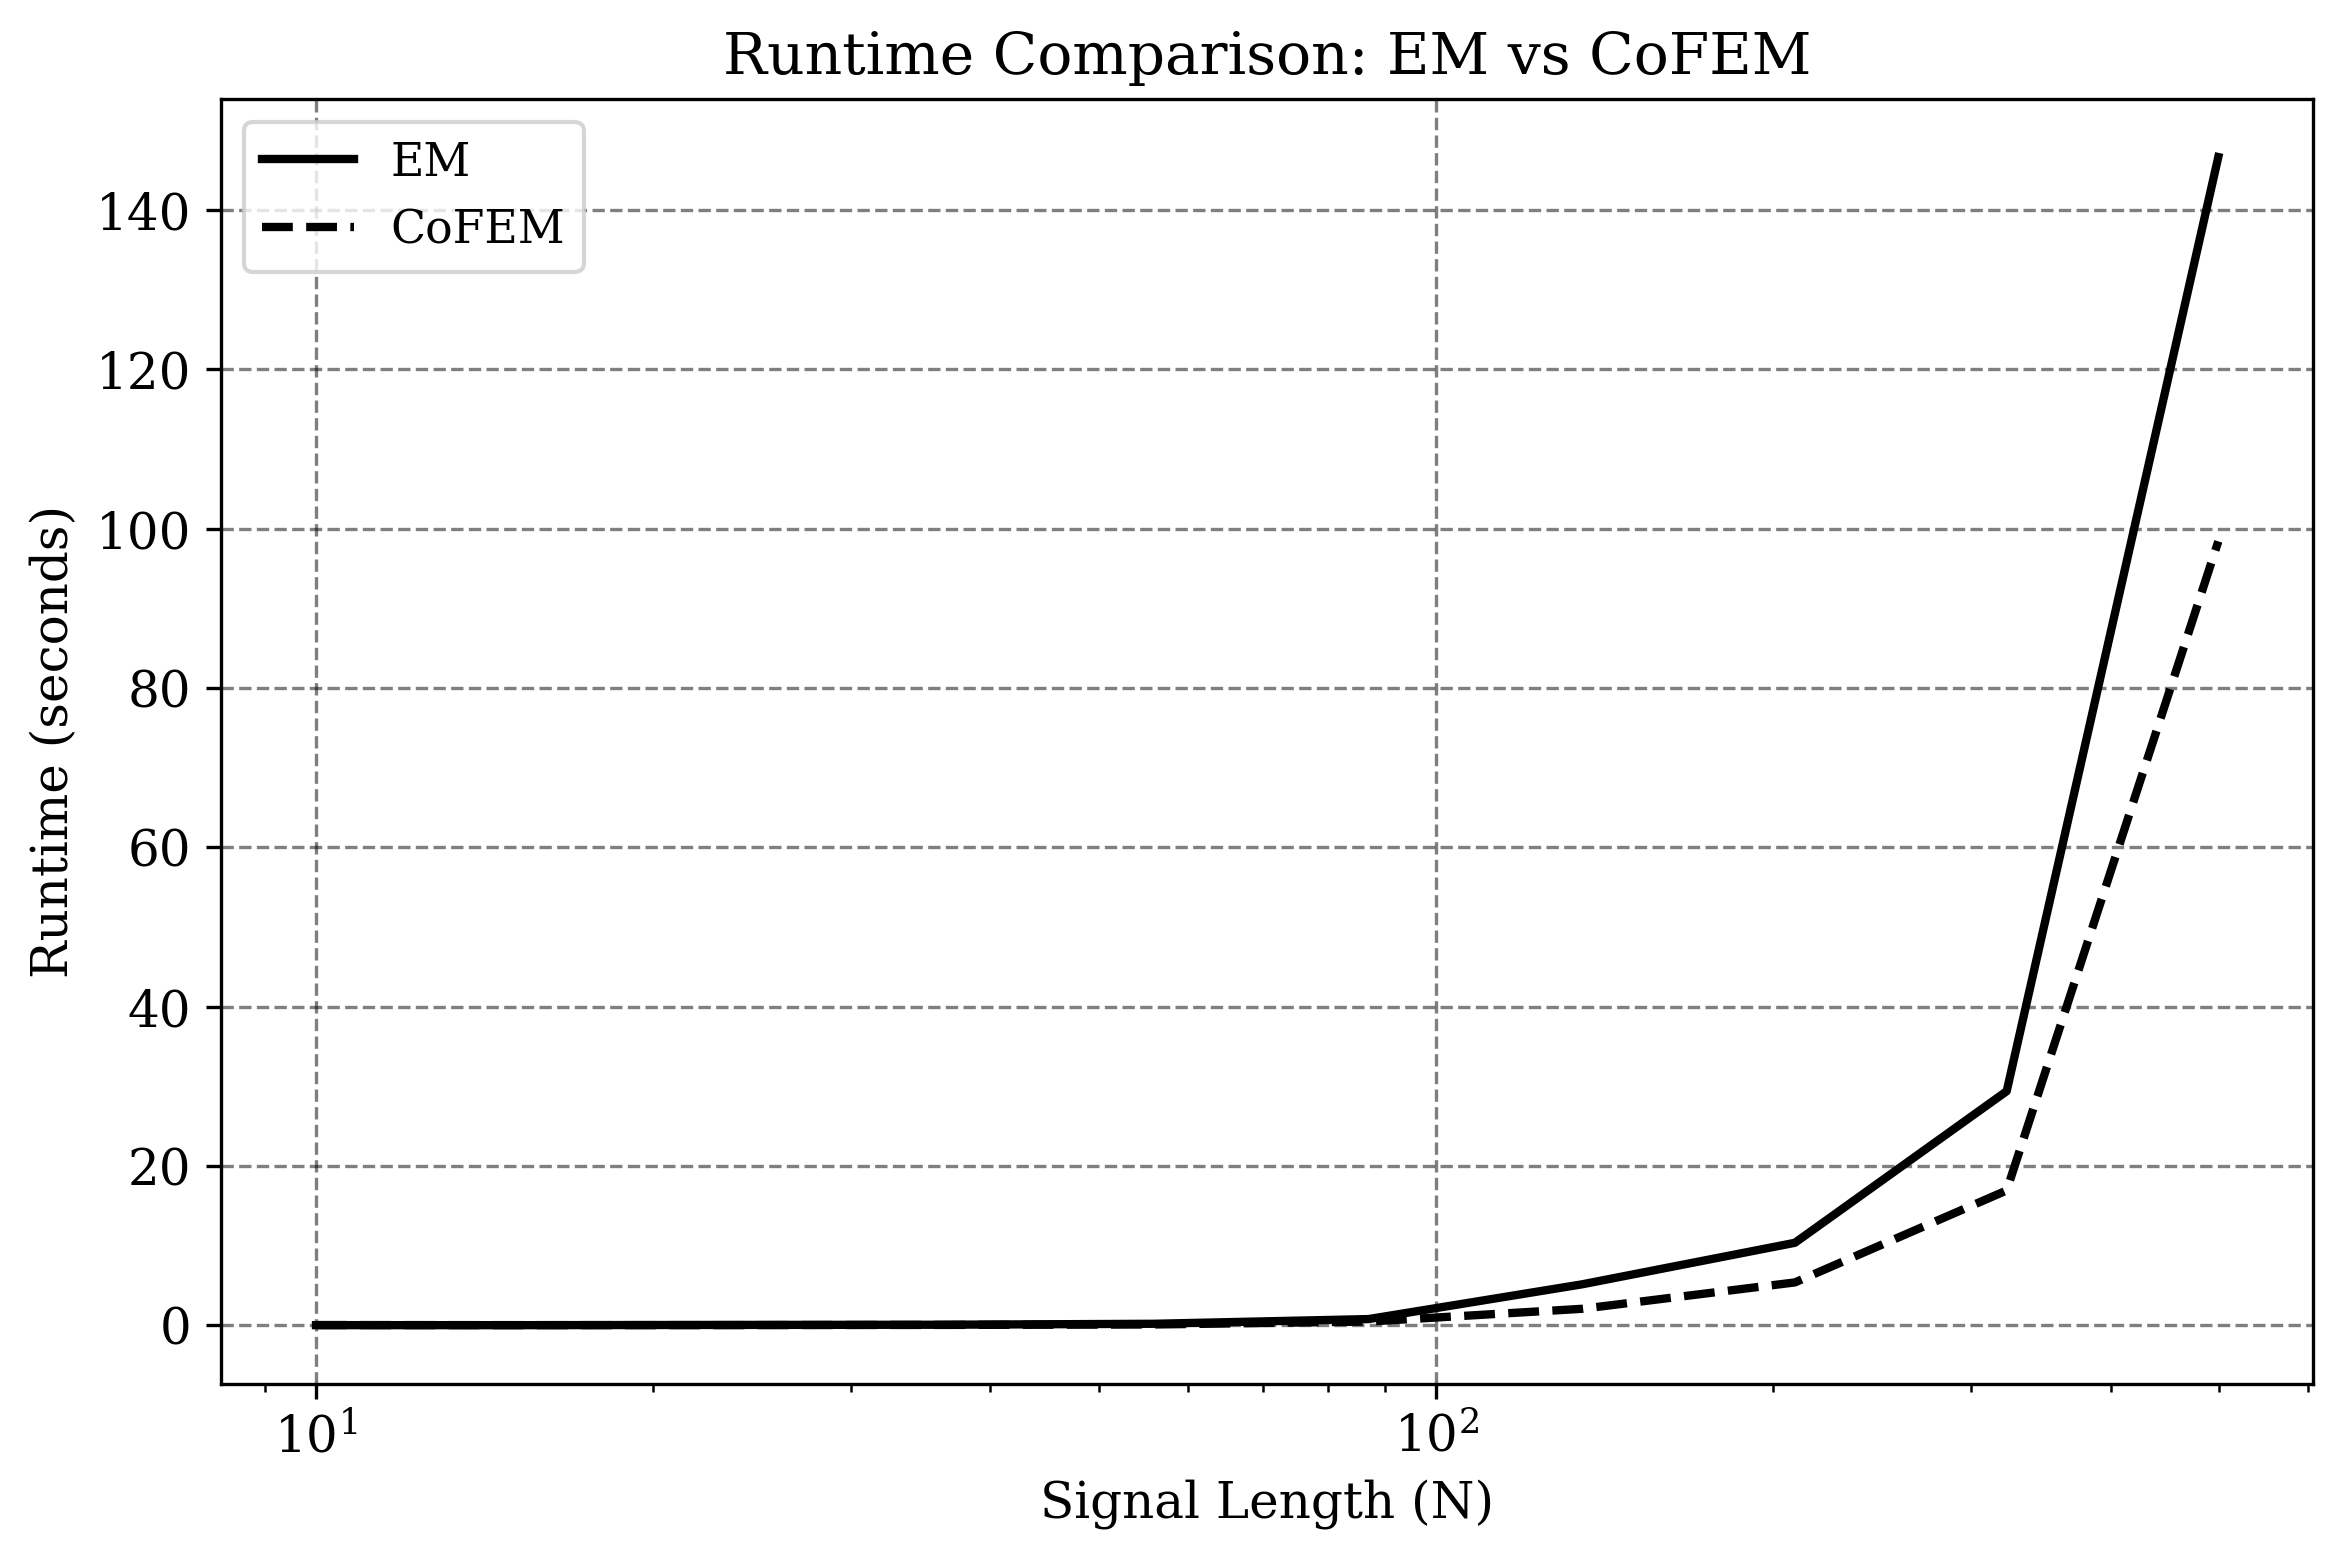
\includegraphics[width=0.8\textwidth]{Figures/runtime_comp.png}
        \caption{Runtime of EM and CoFEM algorithms for increasing measurements $N$. Dictionary size $D=3N$. }
    \end{figure}
\end{frame}

\begin{frame}{Accuracy Comparison: Gaussian Matrices}
    \begin{itemize}
        \item EM and CoFEM exhibited nearly identical reconstruction accuracy in Gaussian measurement systems. 
        \item CoFEM with unknown noise variance performed on par with variants assuming known noise level. 
    \end{itemize}
    \begin{figure}[h!]
        \centering
        \begin{subfigure}[b]{0.48\textwidth}
            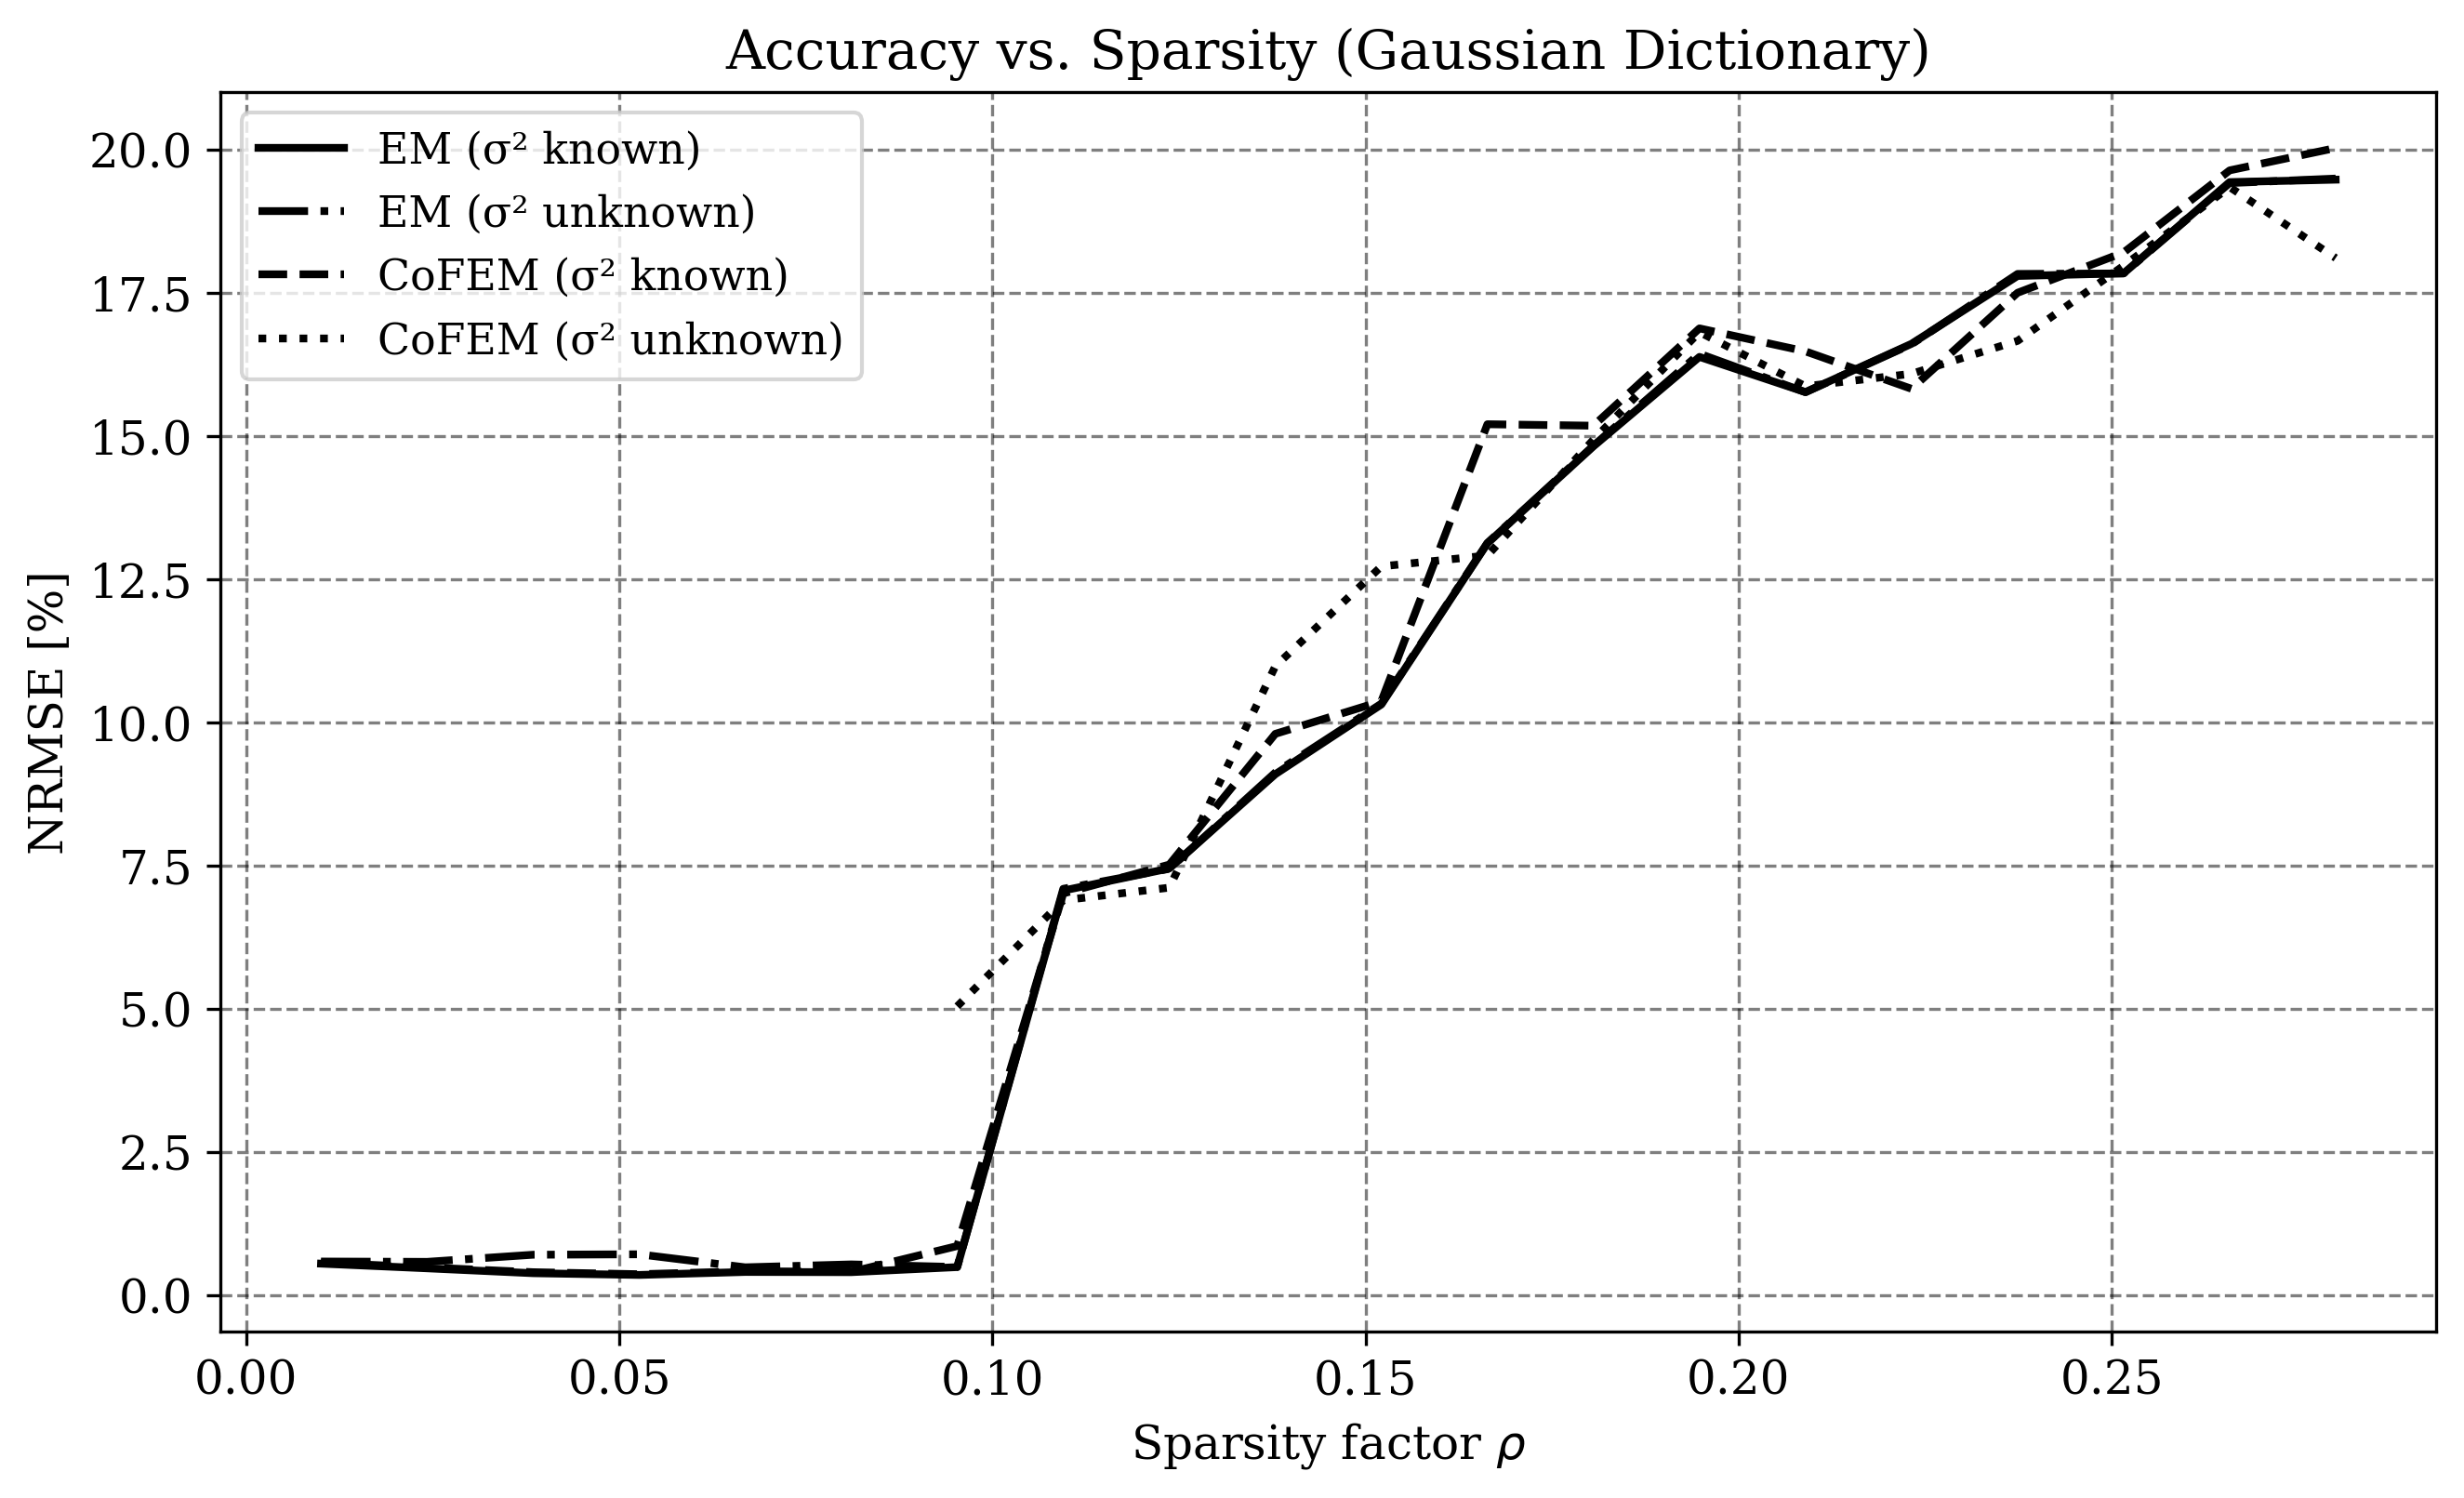
\includegraphics[width=\textwidth]{Figures/accuracy_vs_sparsity_EMCoFEM.png}
            \caption{NRMSE vs. sparsity level $\rho$. }
        \end{subfigure}
        \hfill
        \begin{subfigure}[b]{0.48\textwidth}
            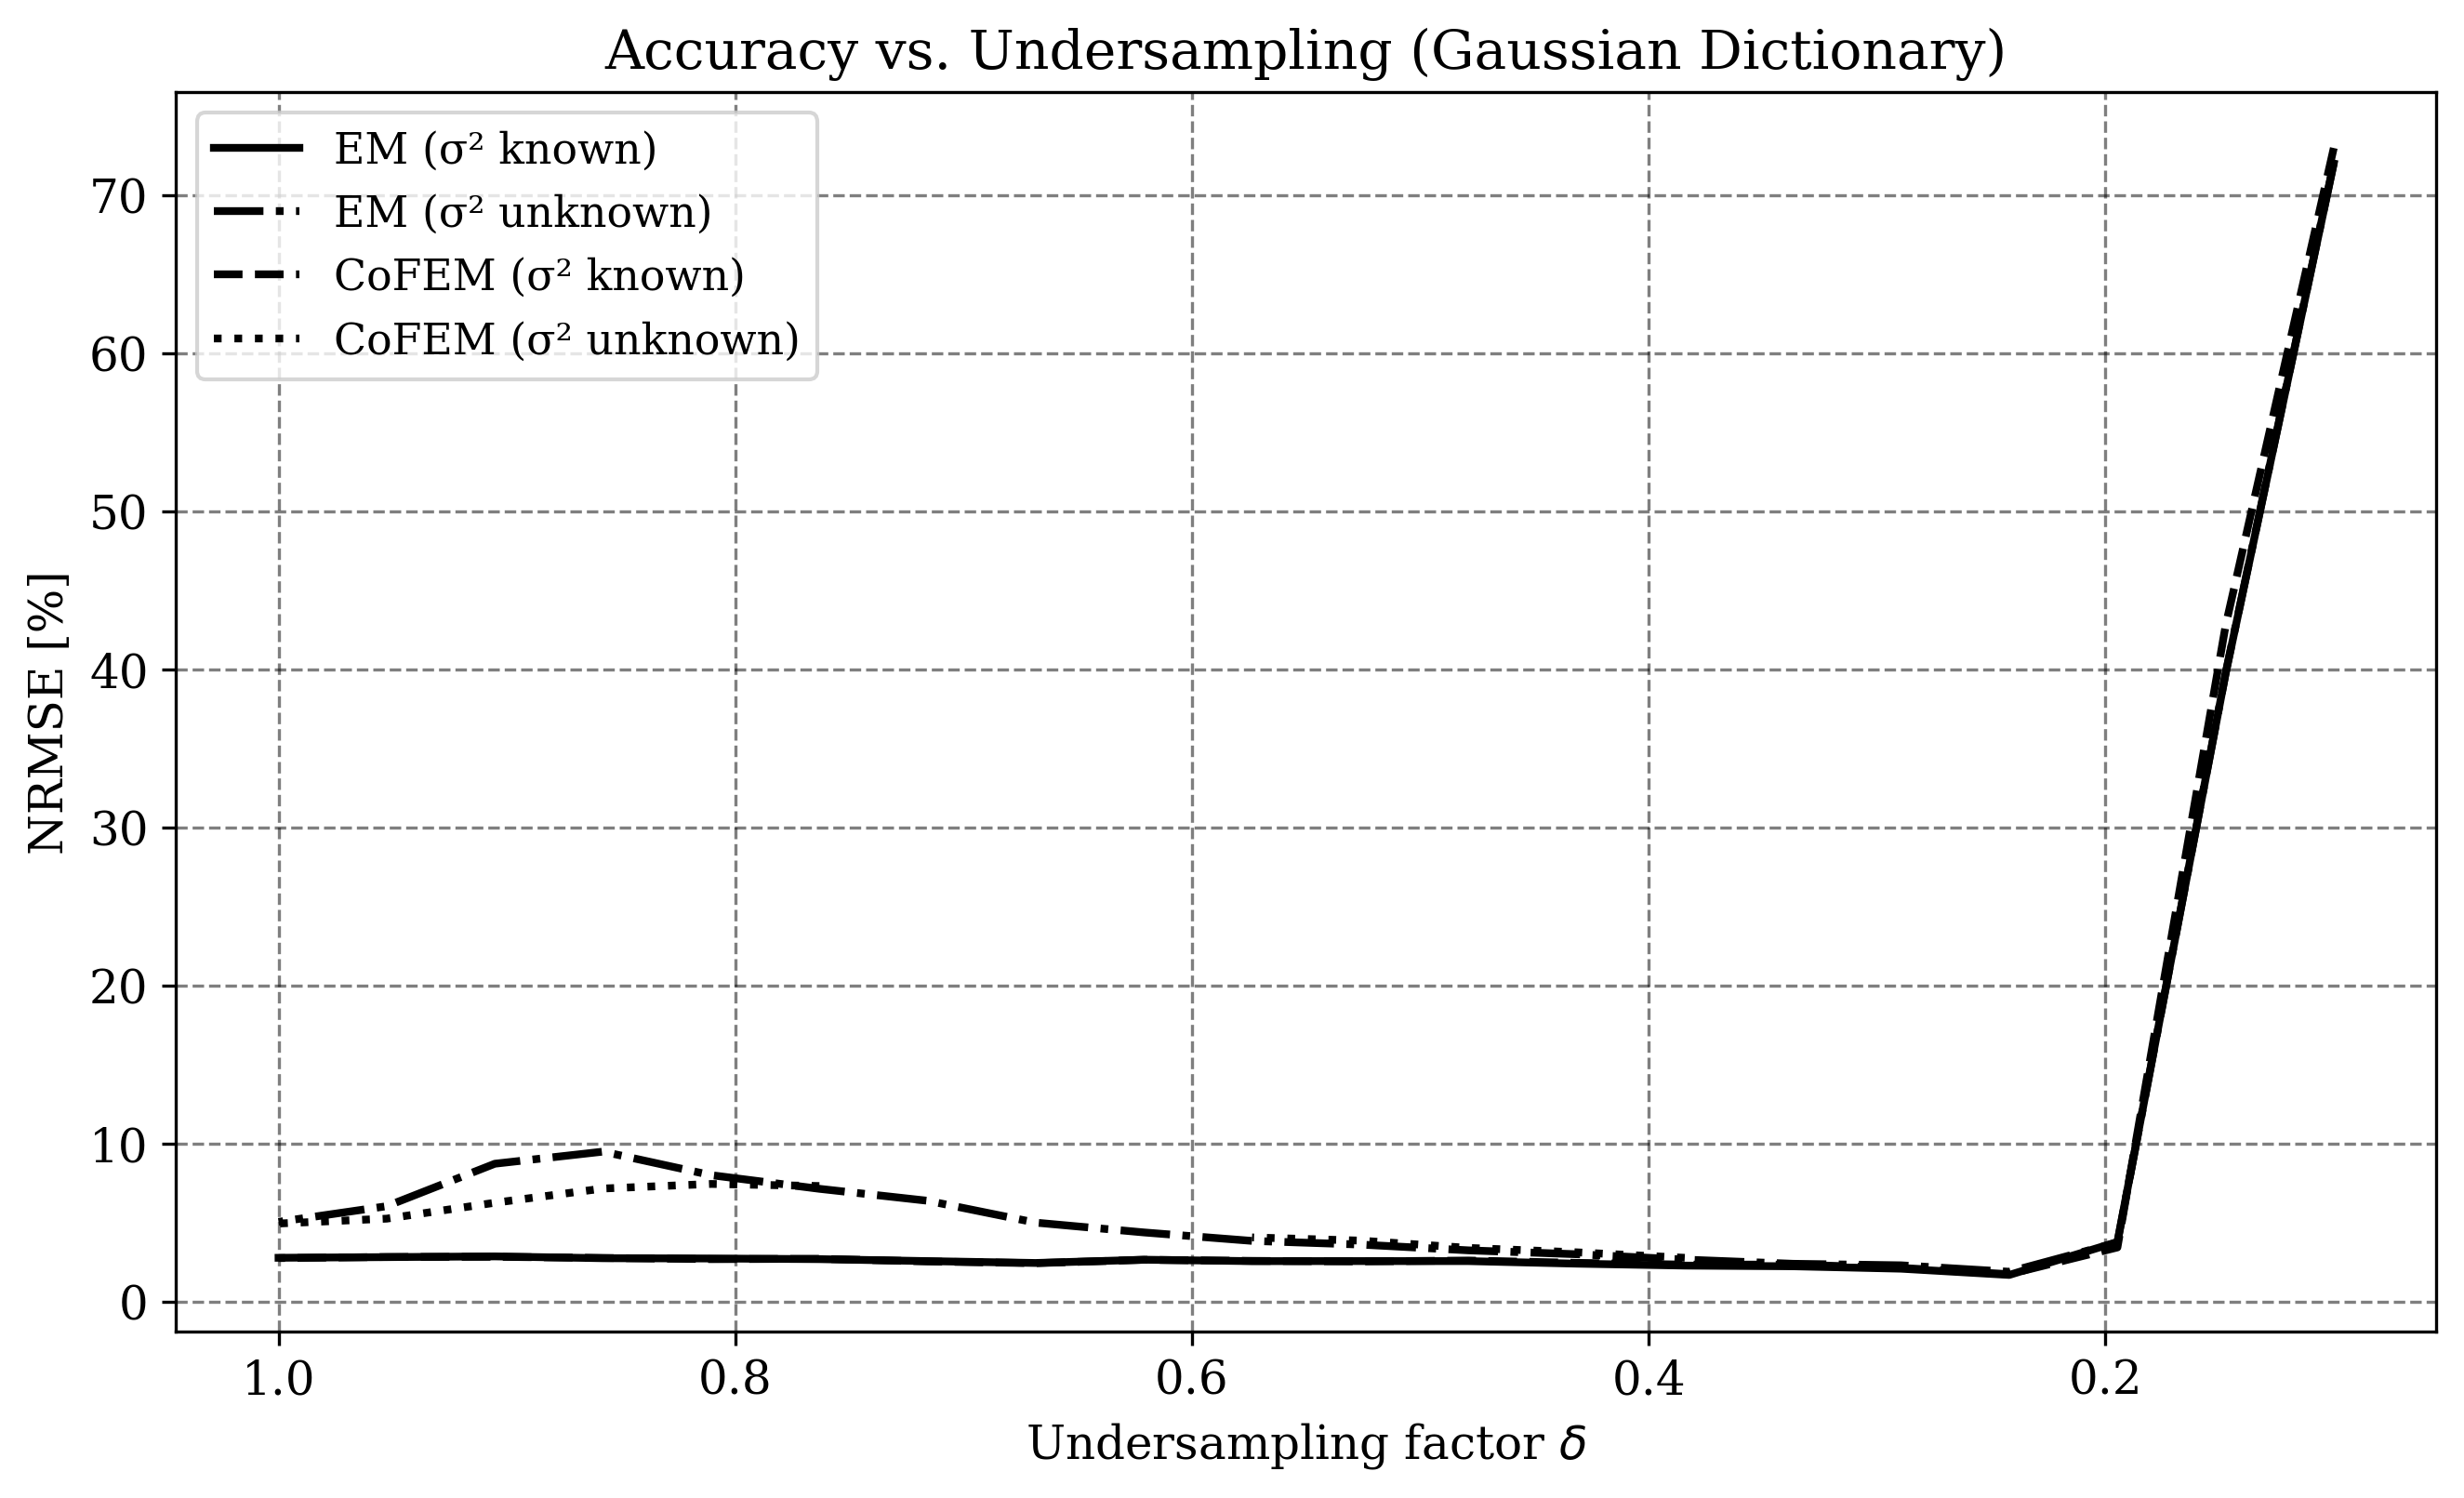
\includegraphics[width=\textwidth]{Figures/accuracy_vs_undersampling_EMCoFEM.png}
            \caption{NRMSE vs. undersampling factor $\delta$. }
        \end{subfigure}
        \caption{Reconstruction accuracy for EM and CoFEM algorithms with Gaussian dictionaries.}
    \end{figure}
\end{frame}

\begin{frame}{Challenges with Fourier Matrices (EM/CoFEM)}
    \begin{itemize}
        \item EM algorithm showed unstable behavior and sensitivity to initialization for complex-valued (FFT-based) dictionaries. 
        \item Efforts to adapt EM for this case were discontinued due to unreliability. 
    \end{itemize}
\end{frame}

\begin{frame}{SBL-SURE (Tipping's FML) Performance}
    \begin{itemize}
        \item Demonstrated robust performance across both Gaussian and complex-valued systems. 
        \item Accuracy in Gaussian systems closely matched EM's, with EM showing marginal improvements. 
        \item \textbf{Key Finding:} In complex-valued systems (Fourier matrices), Tipping's method outperformed its own Gaussian results, suggesting better adaptation to structured dictionaries. 
    \end{itemize}
    \begin{figure}[h!]
        \centering
        \begin{subfigure}[b]{0.48\textwidth}
            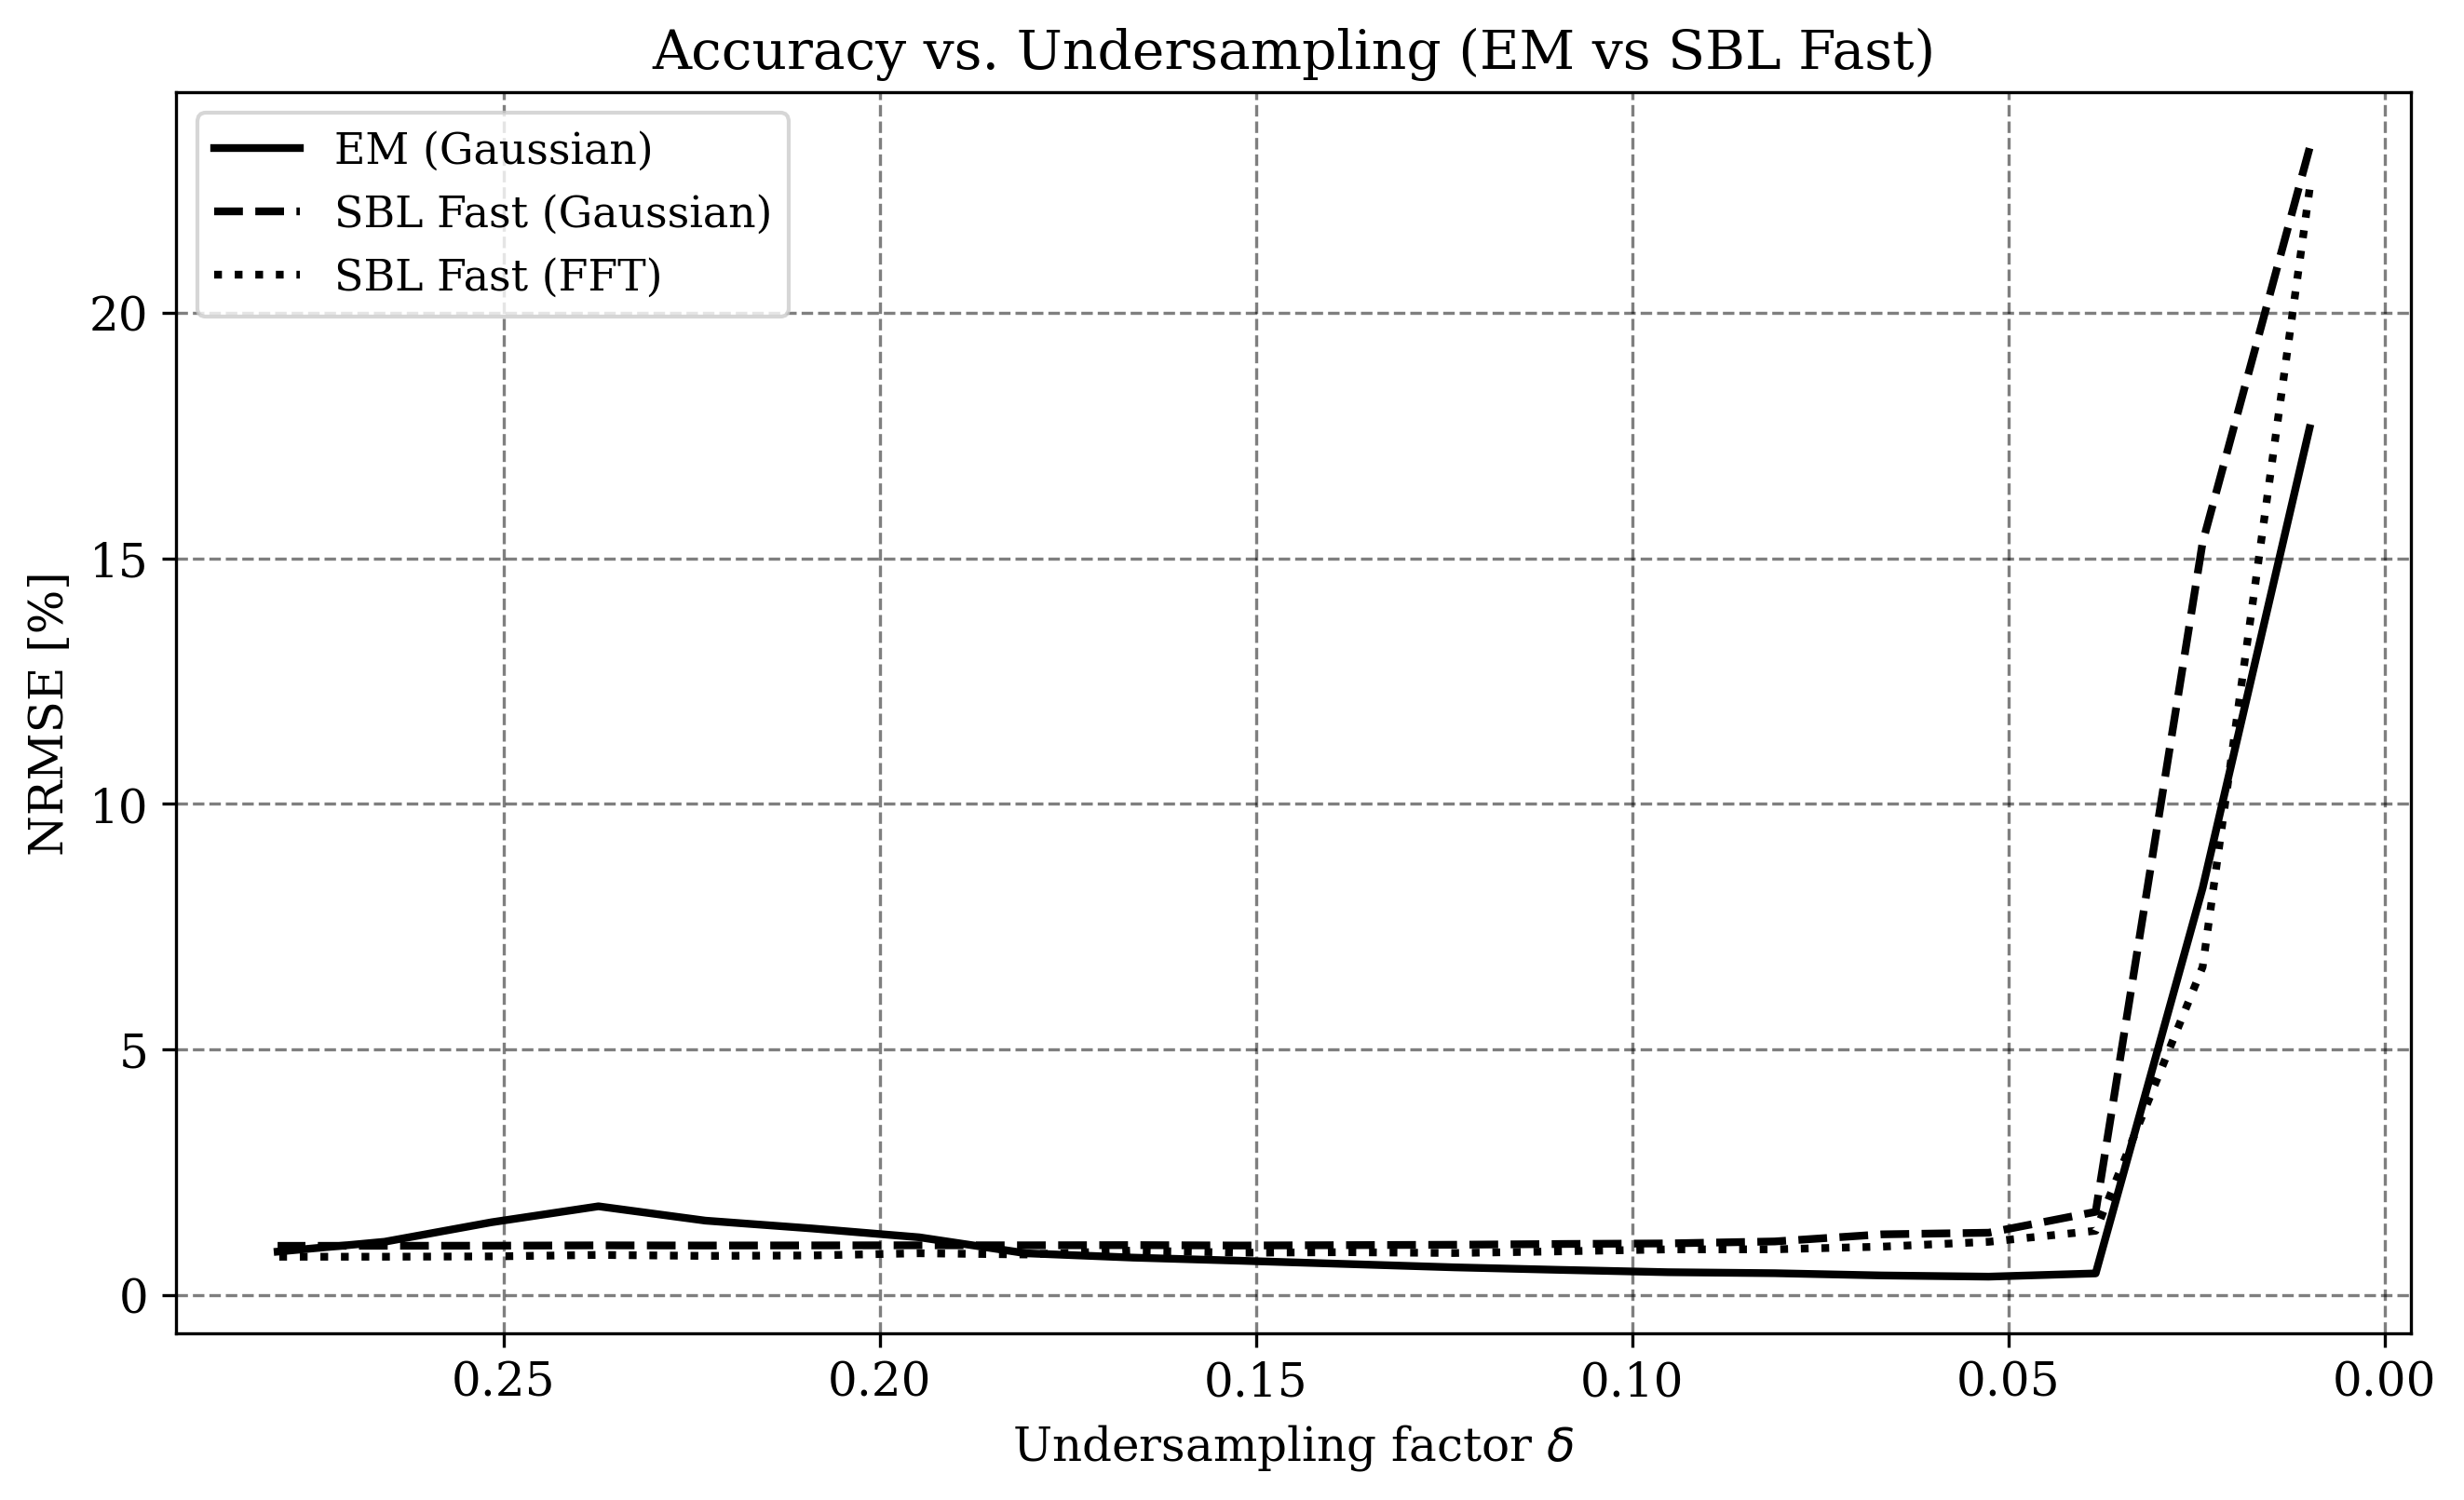
\includegraphics[width=\textwidth]{Figures/accuracy_vs_undersampling_EMvsSB_woEMFFT.png}
            \caption{NRMSE vs. undersampling factor $\delta$. }
        \end{subfigure}
        \hfill
        \begin{subfigure}[b]{0.48\textwidth}
            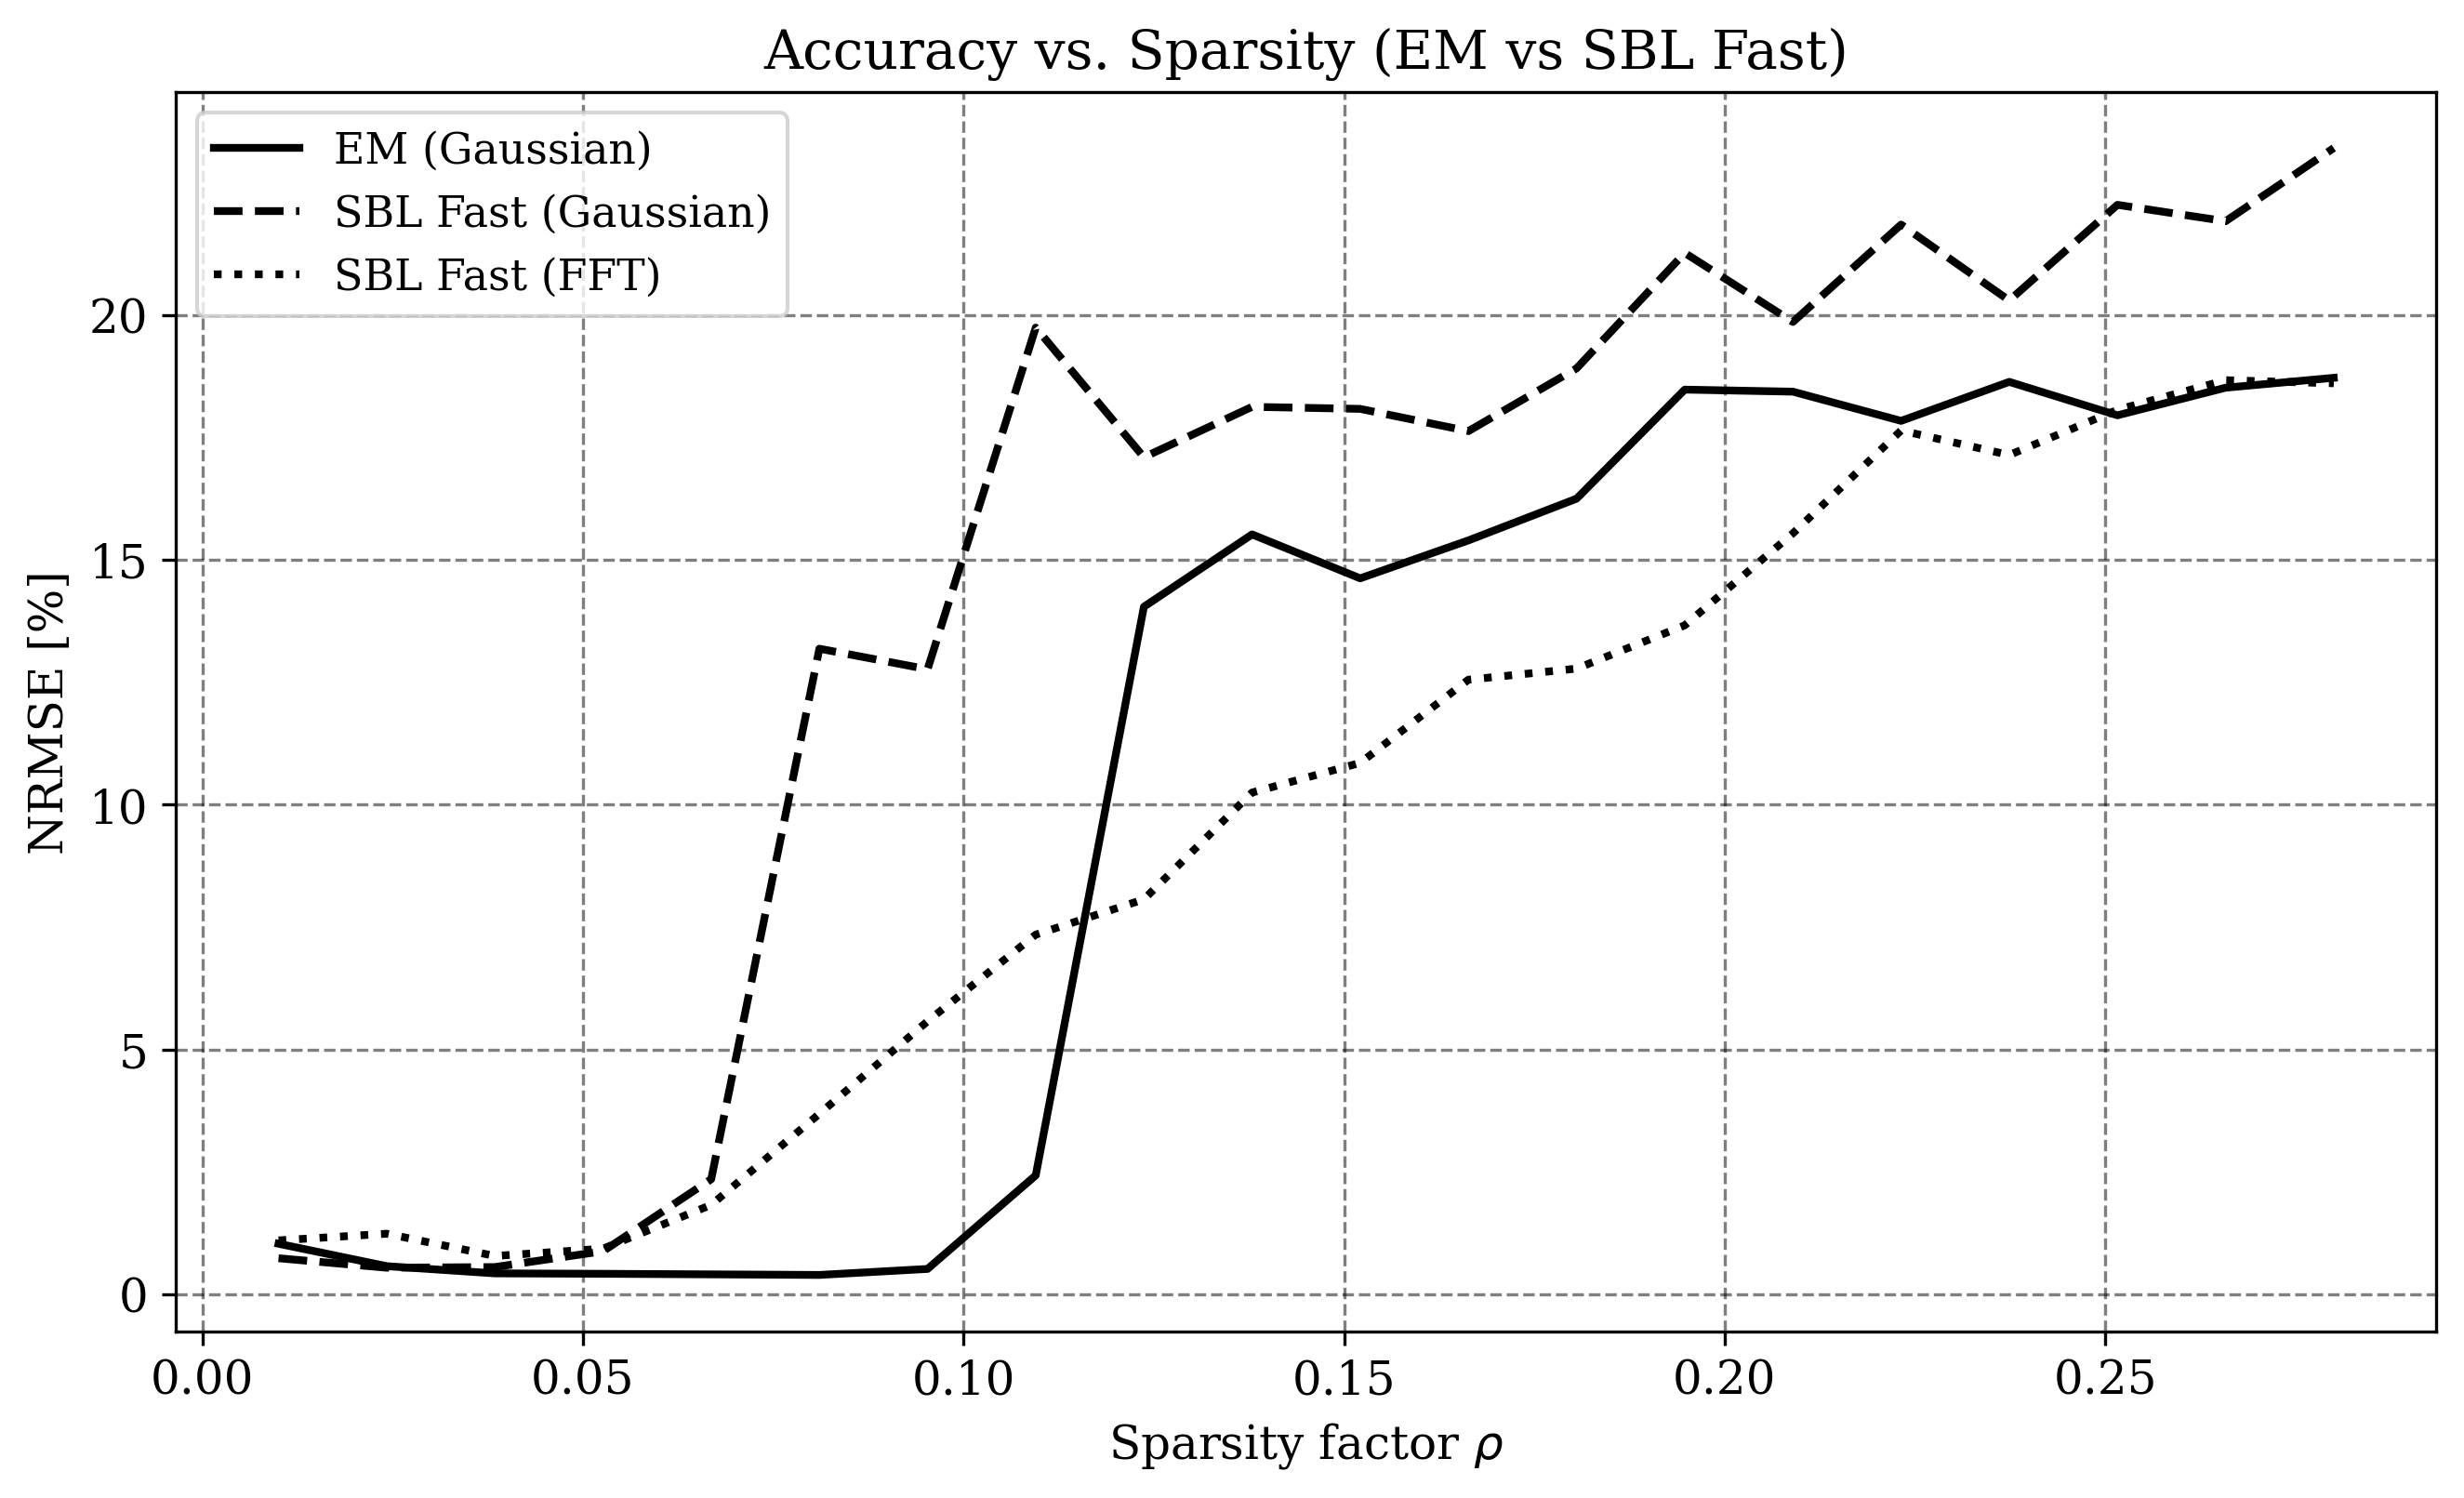
\includegraphics[width=\textwidth]{Figures/accuracy_vs_sparsity_EMvsSB_woEMFFT.png}
            \caption{NRMSE vs. sparsity ratio $\rho$. }
        \end{subfigure}
        \caption{Reconstruction accuracy for Tipping's FML algorithm.}
    \end{figure}
\end{frame}

% Conclusion & Future Work
\section{Conclusion & Future Work}
\begin{frame}{Conclusion}
    \begin{itemize}
        \item Successfully investigated and applied compressive sensing techniques for antenna pattern extrapolation. 
        \item Implemented and evaluated various sparse learning algorithms (EM, CoFEM, SBL-SURE/FML). 
        \item SBL with SURE (Tipping's FML algorithm) proved to be the most robust and efficient method, particularly for structured (Fourier) measurement matrices. 
        \item This work demonstrates the potential of CS methods in improving antenna measurement techniques. 
    \end{itemize}
\end{frame}

\begin{frame}{Future Work}
    \begin{itemize}
        \item Reformulate EM algorithm to reduce computational complexity for high-dimensional problems (e.g., using Woodbury identity). 
        \item Explore further optimization of algorithms for specific antenna models.
        \item Validate findings with real-world antenna measurement data.
        \item Extend the framework to other types of electromagnetic problems.
    \end{itemize}
\end{frame}

% Q&A Slide
\begin{frame}
    \centering
    \textsf{\Huge Questions?}
    \vspace{1cm}
    \textsf{\Large Thank you!}
\end{frame}

\end{document}
